\chapter{Vizualizacija}

Ljudje smo naravno nadarjeni za iskanje vzorcev. To počnemo od rojstva, ko moramo odkriti povezavo med tem, kar vidimo in otipamo, ko se naučimo razbirati zvoke, prepoznamo zvezo med besedami ter osebami, dejanji, rečmi, ki jih besede pomenijo\ldots

Po drugi strani so podatki, s katerimi delamo, pogosto v obliki ogromne tabele, navadno ogromne tabele številk, torej natančno v obliki, ki nam je tuja. Če hočemo v teh podatkih kaj odkriti, lahko uporabimo avtomatske metode odkrivanja, kot so gručenje, razvrščanje, povezovalna pravila, ali pa spremenimo podatke v obliko, v katerih bomo lahko vzorce odkrili sami, s svojimi vgrajenimi mehanizmi. Najpreprostejša pot je vizualizacija podatkov.

\begin{table}{htbp}
\begin{tabular}{rcccccccccccc}
& {\bf Jan} & {\bf Feb} & {\bf Mar} & {\bf Apr} & {\bf Maj} & {\bf Jun} & {\bf Jul} & {\bf Avg} & {\bf Sep} & {\bf Okt} & {\bf Nov} & {\bf Dec} \\
{\bf USD} & 1,4149 & 1,3756 & 1,3496 & 1,3379 & 1,3089 & 1,2164 & 1,2119 & 1,2797 & 1,2597 & 1,3542 & 1,3611 & 1,2908 \\
{\bf GBP} & 0,8734 & 0,8621 & 0,8903 & 0,8802 & 0,855 & 0,8397 & 0,8111 & 0,8211 & 0,8184 & 0,8604 & 0,8541 & 0,8284 \\
{\bf YEN} & 130,7238 & 123,5724 & 119,7231 & 124,5692 & 123,4963 & 110,455 & 106,6947 & 110,5044 & 105,7866 & 112,5476 & 109,9054 & 107,3263
\end{tabular}
\caption{Vrednosti različnih valut v primerjavi z evrom v letu 2010}
\label{t-valute}
\end{table}

V Tabeli~\ref{t-valute} lahko vidimo, kakšna je bila vrednost posamezne valute (proti evru) v posameznem mesecu v 2010. Z njo lahko odgovarjamo na vprašanja, kot je ``kaj se je dogajalo z vrednostjo dolarja'', težko pa je videti, recimo, ``ali dolar in jen
padata in rasteta hkrati'' ali ``kateri par valut se obnaša podobno”.
Razlog je v tem, da je v delovnem pomnilniku (to ni isto kot kratkoročni spomin!) prostora za tri enote informacije naenkrat. Za odgovor na prvo vprašanje naš delovni pomnilnik
zadošča, za drugi dve pa bi morali primerjati (pre)več številk naenkrat.

Vendar ``tri enote informacije'' ne pomenijo nujno treh številk – lahko so tudi tri krivulje, kakršne vidimo na Sliki~\ref{f-valute} in s katerimi lahko odgovarjamo tudi na drugo in tretje vprašanje (kolikor je odgovor pač nedvoumen).

\begin{figure}[htbp]
\begin{center}
\includegraphics[]{slike/value.png}
\caption{Gibanje vrednosti različnih valut v primerjavi z evrom v letu 2010}
\label{f-valute}
\end{center}
\end{figure}

Pri vizualiziranju podatkov se moramo torej zavedati njenega pomena: podatke vizualiziramo zato, da bi iz slike razbrali več, kot razberemo iz golih številk. Primer, ko je to pravilo kršeno, je t.i. ``Dashboard''\footnote{Imena vizualizacij bomo načelno poskušali prevajati; tale ni vredna truda.}. Primer kaže Slika~\ref{f-dashboard}. Vizualizacija kaže devet števil, ki niso povezane (v tem smislu, da bi predstavljale deleže česa ali spremembe v času ali kaj podobnega). V tem primeru bi bilo veliko preprosteje preprosto napisati deset številk.

\begin{figure}[htbp]
\begin{center}
\includegraphics[]{slike/dashboard.png}
\caption{Primer nepotrebne vizualizacije}
\label{f-dashboard}
\end{center}
\end{figure}

Obenem je oblika vizualizacija zavajajoča, saj sugerira, na primer, da je ``možno'' število ocenjevalcev patentov med 6400 in 7400; trenutno smo nekje na sredini. Kaj pa se zgodi, ko število preseže 7400? Obstaja morda kak zakonski predpis, da čakalna vrsta ne sme presegati enega milijona?

Za sestavljanje dobrih vizualizacij, kadar so te potrebno, moramo upoštevati določena pravila.

V spominu ni prostora za dve sliki hkrati. Če hočemo primerjati dve sliki, lahko to počnemo le ta, da izmenično gledamo eno in drugo, pri čemer si moramo zapomniti detajl z ene slike in ga iskati na drugi.

!!!! turisti

Pri gledanju slik imamo določena pričakovanja. Stvari, ki jih ne pričakujemo, pogosto ne bomo videli in, obratno, kadar pričakujemo, da bomo videli določen vzorec, to poveča verjetnost, da ga bomo v resnici opazili.

!!!! slike šuma

!!!! delfini

Obstajajo tudi konvencije o tem, kako gledamo slike. Čas vedno teče od leve proti desne, ne obratno. Podobno naraščajo druge vrednosti. Če narišemo graf, ki teče v nasprotni smeri, ga bomo težko gledali, saj nam bo obračanje vzelo toliko "možganske moči", da je ne bo dovolj za analizo slike. Prav tako obstajajo konvencije o barvah: zeleno je dobro, rdeče slabo ali nevarno. Moški smo modri, ženske roza. Japonska je oranžna in Francija zelena.

Različnih standardnih vizualizacij je v resnici malo; večina galerije vizualizacij v programih, kot je Excel, so le variacije na par različnih tem.

\section{Tortni diagrami}

Tortni diagrami so ena najpogostejših vizualizacij, a obenem praktično neuporabni. V osnovi so namenjeni prikazovanju diskretnih porazdelitev, torej deležev, ki se seštejejo v 1 oziroma v 100\%.

Izkaže se, da takšnih podatkov pogosto ni potrebno risati. Namen slike je, da nam razkrije kaj, česar brez nje ne bi vedeli. Za primer nepotrebnega grafa privzemimo, da je neka trgovina odkrila, da je 60 % njenih strank žensk. Da bi bila stvar očitnejša, narišejo še sliko (Slika\ref{f-pie1-2d}).

\begin{figure}[H!]
\begin{center}
\subfigure{}{Primer nepotrebnega tortnega diagrama\label{f-pie-2d}}{
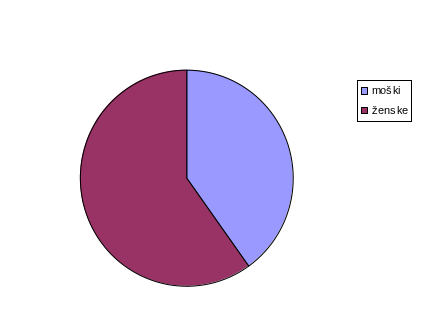
\includegraphics[width=0.45\textwidth]{slike/pie2d.png}
}
\subfigure{}{Primer nepotrebnega tortnega diagrama v treh dimenzijah\label{f-pie-3d}}{
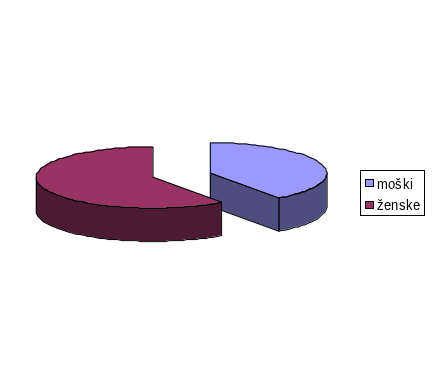
\includegraphics[width=0.45\textwidth]{slike/pie3d.png}
}
\end{center}
\end{figure}

Če želijo sliko še izboljšati, jo bodo postavili ``v tri dimenzije'' (Slika\ref{f-pie-3d}), ki ji Excel pravi ``Exploded pie with a 3-D visual effect''.

Kaj nam pove več: številka ali slika? Gotovo številka. Vsi vemo, kaj je to 60% - med desetimi strankami je šest žensk. Med petimi so tri. Kaj pa pove diagram? More kdo iz "eksplodirane torte" razbrati, koliko je žensk? Razen tega, da jih je nekaj več kot moških?
Težavo bi seveda delno rešili s tem, da bi na sliko dodali številko. Vendar bi bilo prav tako vseeno, če bi celotno torto zamenjali s številko ali dvema.

BBC je na spletnih straneh, namenjenih učenju branja grafov, objavil biser na Sliki\ref{f-pie-bbc}. Prvi graf kaže delež časa, ki ga v poprečju preživimo ob branju časopisov, leposlovja, revij\ldots Celotna torta predstavlja ves čas, ki ga posvetimo branju, in torto razrežemo na dele, ki ustrezajo posamezni vrsti branja. Deleže, ki jih kaže torta, v mislih pretvarjamo v četrtine, tretjine... mar ne bi bilo potem boljše, če bi nam avtorji pokazali kar številke?

\begin{figure}[htbp]
\begin{center}
\includegraphics[]{slike/pie-bbc.png}
\caption{Primer napačne rabe tortnih diagramov}
\label{f-pie-bbc}
\end{center}
\end{figure}

Spodnji graf na Sliki\ref{f-pie-bbc} pa res nima smisla, saj kaže to so deleže ... česa?! Deleži izmed
razpoložljivega časa vseh zdravnikov (GP je splošni zdravnik) teh šestih evropskih
držav, ki jih namenijo državljanom posamezne države? Če gre v resnici za
poprečne čase, ki jih državljani teh držav preživijo pri splošnih zdravnikih, bi bilo
boljše narisati stolpčni diagram (bar chart).

\begin{figure}[htbp]
\begin{center}
\includegraphics[]{slike/pie-bbc.png}
\caption{Primer napačne rabe tortnih diagramov}
\label{f-pie-bbc}
\end{center}
\end{figure}

Celo, kadar so narejeni pravilno, tortni diagrami ne kažejo veliko, saj so nerodni. Iz torte na sliki~\ref{f-allocations-a} ne moremo razbrati deležev (še posebej, ker je
nagnjena, a tudi, če ne bi bila, bi bilo težko). Barve so nepregledne, ker so si (vsaj
zelene) preveč podobne. Za branje tortnega diagrama je potrebno
stalno gledati v legendo. Dobri tortni diagrami so takšni, kjer so oznake ob
diagramu. Vendar za to navadno ni dovolj prostora; če ga je, pa oznak verjetno ni
veliko in bi več povedala tabela.

Tule so se tega zavedali, zato so dodali tabelo; ta pove več kot slika, žal pa je nerodno urejena.
Tortne diagrame navadno vedno lahko zamenjamo kar s takšnimi tabelami. Grafično pa bi taiste podatke bi bilo mogoče veliko lepše narisati tako, kot kaže slika~\ref{f-allocations-b.}

Na Sliki~\ref{f-sothebys} je prikazano spreminjanje tržnih deležev hiš Sotheby's in Christie's. Brez številk ne pove ničesar... brez tort pa ne bi pogrešali ničesar.

Tortne diagrame je težko primerjati med seboj. Spomnimo se: če želimo primerjati dve sliki, lahko to storimo le tako, da s pogledom skačemo od ene do druge in primerjamo detajle. Da odgovorimo na vprašanje, katera etnična skupina v ZDA ima največji delež krvne skupine B (Slika~\ref{f-krvne-skupine}), moramo nekaj časa skakati s pogledom od enega do drugega grafa. Veliko boljše je uporabiti palični diagram, kot ga kaže Slika~\ref{f-krvne-skupine-pslice}.

Tortnim diagramom se torej v splšnem izogibajmo, saj so pretežno neuporabni.


